% === T19 - Almacenamiento Masivo ===
% David Alejandro Gonzalez Marquez
% fokerman@gmail.com
% https://github.com/fokerman/computingSystemsCourse

\RequirePackage[2020-02-02]{latexrelease}

\documentclass[aspectratio=169]{beamer}
\usepackage{../packages}

\title{\Huge Almacenamiento Masivo}
\author{David Alejandro González Márquez}
\institute{}

\date{}

\begin{document}

\begin{frame}[plain]
    \titlepage
    \begin{textblock}{100}(30,80)
    \begin{tcolorbox}[size=small,width=\textwidth,colback={gray!30},title={}]
    \begin{center}
     \scriptsize Clase disponible en: \url{https://github.com/fokerman/computingSystemsCourse}
    \end{center}
    \end{tcolorbox}
    \end{textblock}
\end{frame}

\begin{frame}{Almacenamiento Masivo}
    En todo sistema necesitamos almacenar datos que perduren en el tiempo,\\ incluso después que el sistema deja de tener energía.\\
    \bigskip
    Estos se denominan \textbf{Sistemas de Almacenamiento Secundario}\\ o \textbf{Sistemas de Almacenamiento Masivo}.\\
    \bigskip
    \pause
    \textcolor{naranjauca}{Conceptos}\\
    \small
    \begin{itemize}
    \item[-] \textbf{Sistema de Archivos}\\ Organización lógica de la información en bloques de almacenamiento secundario.
    \item[-] \textbf{Sistemas de almacenamiento}\\ Organización del espacio de almacenamiento y su forma de acceder.
    \item[-] \textbf{Tecnologías de almacenamiento}\\ Hardware específico para implementar sistemas de almacenamiento.
    \item[-] \textbf{Tecnologías de conexionado}\\ Buses, protocolos y conectores físicos se utilizan para contactar dispositivos.
    \end{itemize}
\end{frame}

\begin{frame}[t]{Tecnologías de discos}
    Existen distintos tipos de tecnologías de almacenamiento secundario.\\
    \begin{textblock}{100}(10,20)
    \uncover<2->{
    \textcolor{naranjauca}{\textbf{Discos magnéticos}} o \textcolor{naranjauca}{\textbf{HDDs}} (\textit{Hard Disk Drives})\\
    \small
    Está compuestos por discos recubiertos de material magnético que giran a una velocidad de entre 5400 a 15000 RPM.
    Sobre estos discos un brazo se posiciona y escribe o lee información. }
    \end{textblock}
    \begin{textblock}{100}(10,40)
    \uncover<3->{
    \textcolor{naranjauca}{\textbf{Discos de estado sólido}} o \textcolor{naranjauca}{\textbf{SSDs}} (\textit{Solid-State Drives})\\
    \small
    Son un arreglo de memorias tipo \texttt{flash}, que para evitar el desgaste por reiteradas escrituras cuentan con una capa de traducción.
    Esta capa virtualiza el espacio de escritura, permitiendo que todas las escrituras nuevas se realicen sobre bloques diferentes del disco. }
    \end{textblock}
    \begin{textblock}{100}(10,64)
    \uncover<4->{
    \textcolor{naranjauca}{\textbf{Cintas magnéticas}} o \textcolor{naranjauca}{\textbf{LTO}} (\textit{Linear Tape-Open}) o \textcolor{naranjauca}{\textbf{DLT}} (\textit{Digital Line Tape})\\
    \small
    Usan cartuchos de cintas que por medio de un cargador permiten ser escritas y leídas de forma secuencial.
    Tienen gran capacidad y un costo muy reducido. En general se utilizan para grandes \emph{backups}. }
    \end{textblock}
    \begin{textblock}{75}(120,15)
    \uncover<2->{ 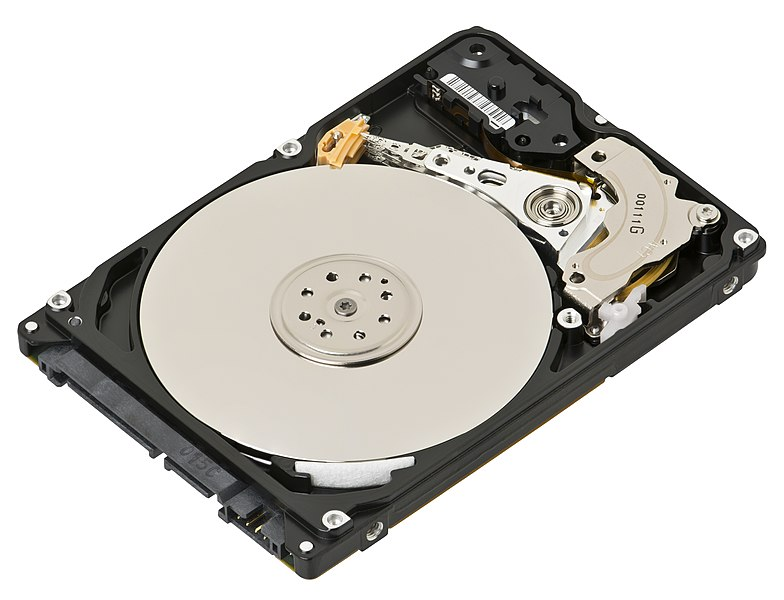
\includegraphics[width=3.2cm]{img/hdd-inside.jpg} }
    \end{textblock}
    \begin{textblock}{75}(120,40)
    \uncover<3->{ \scalebox{-1}[1]{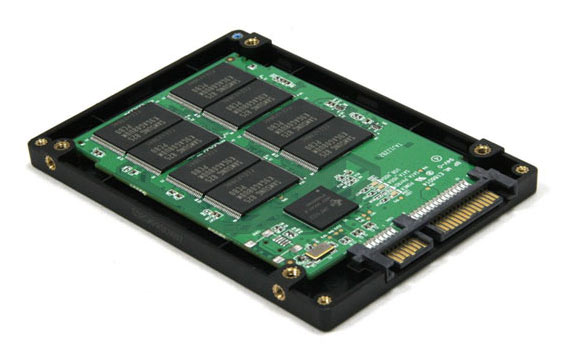
\includegraphics[width=3.2cm]{img/ssd-inside.jpg}} }
    \end{textblock}
    \begin{textblock}{75}(120,60)
    \uncover<4->{ 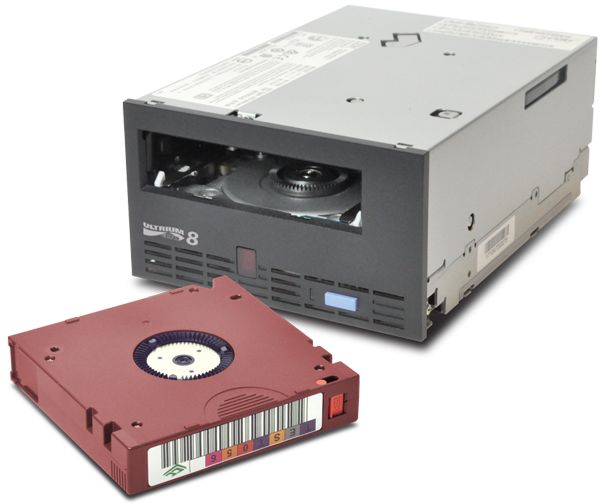
\includegraphics[width=3.2cm]{img/lto-8.png} }
    \end{textblock}
%     \textcolor{naranjauca}{\textbf{Discos de RAM}} o \textcolor{naranjauca}{\textbf{RAMdisk}} (\textit{RAM Disk Drives}).\\
%     Se implementan por medio de placas conectadas directamente al bus de entrada/salida. Estas placas son un arreglo de memorias tipo RAM.
%     Si bien lo consideramos un tipo de disco, porque se utiliza como interfaz, su almacenamiento es volatil, a diferencia de los anteriores.
\end{frame}

\begin{frame}{Discos magnéticos}
    \begin{textblock}{75}(92,40)
    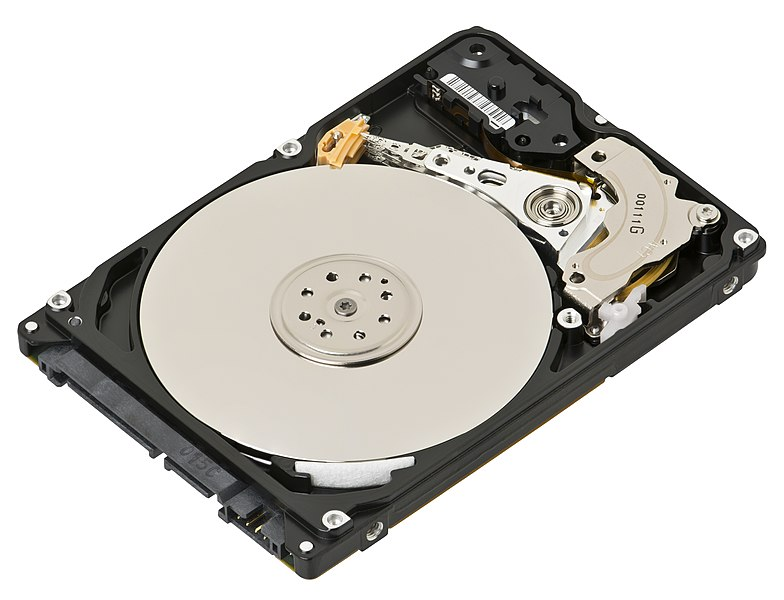
\includegraphics[width=6.2cm]{img/hdd-inside.jpg}
    \end{textblock}
    \begin{textblock}{100}(80,5)
    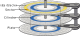
\includegraphics[scale=0.9]{img/discos.pdf}     
    \end{textblock}
    \begin{textblock}{70}(7,15)
    \small
    En general los discos se organizan en \textbf{cilindros}, \textbf{pistas} y \textbf{sectores}.\\
    \bigskip
    \uncover<2->{
    En los primeros discos la controladora solo podía ubicar un sector, leerlo o escribirlo de forma serial.
    Delegando toda la inteligencia al software.\\ }
    \bigskip
    \uncover<3->{
    Los discos modernos contienen microcontroladores que permiten exponer una interfaz de más alto nivel.
    Se ocupan de presentar un \textbf{espacio lineal de direccionamiento} y resolver problemas de \textbf{reasingnación de bloques} en el caso de falla.\\ }
    \bigskip
    \uncover<4->{
    Además contienen dispositivos DMA integrados junto con memorias que usan como \textbf{buffers de bloques}.\\ }
    \end{textblock}
\end{frame}

\begin{frame}{Discos magnéticos}
    \begin{textblock}{100}(80,2)
    \uncover<4->{ \includegraphics[trim={1cm 11.19cm 6.91cm 4.2cm},clip,scale=0.6,page=2]{img/barracuda-2-5-DS1907-3-2005LA-es_LA.pdf} }
    \end{textblock}
    \begin{textblock}{100}(68,2)
    \uncover<4->{ \textcolor{verdeuca}{\textbf{Ejemplo:}} }
    \end{textblock}
    \begin{textblock}{70}(7,15)
    \small
    El plato en los discos gira a una velocidad fija, esto permite calcular con mucha precisión el flujo de lectura y escritura de los datos.\\
    \bigskip
    \uncover<2->{
    Estas velocidades pueden ser de 4800 RPM, 5400 RPM, 7200 RPM o incluso llegar a velocidades de 15000 RPM.\\ }
    \bigskip
    \uncover<3->{
    \textcolor{verdeuca}{Algunas características físicas en discos} 
    \begin{itemize}
    \setlength\itemsep{0cm}
    \item[-] Tiempo de búsqueda \emph{(seek time)}
    \item[-] Latenia rotacional \emph{(rotational latency)}
    \item[-] Velocidad de transferencia \emph{(transfer rate)}
    \item[-] Velocidad de posicionamiento \emph{(positioning time)}
    \end{itemize}
    }
    \end{textblock}
\end{frame}

\begin{frame}{Discos de estado sólido (NVM)}
    \begin{textblock}{100}(15,60)
    \uncover<4->{ 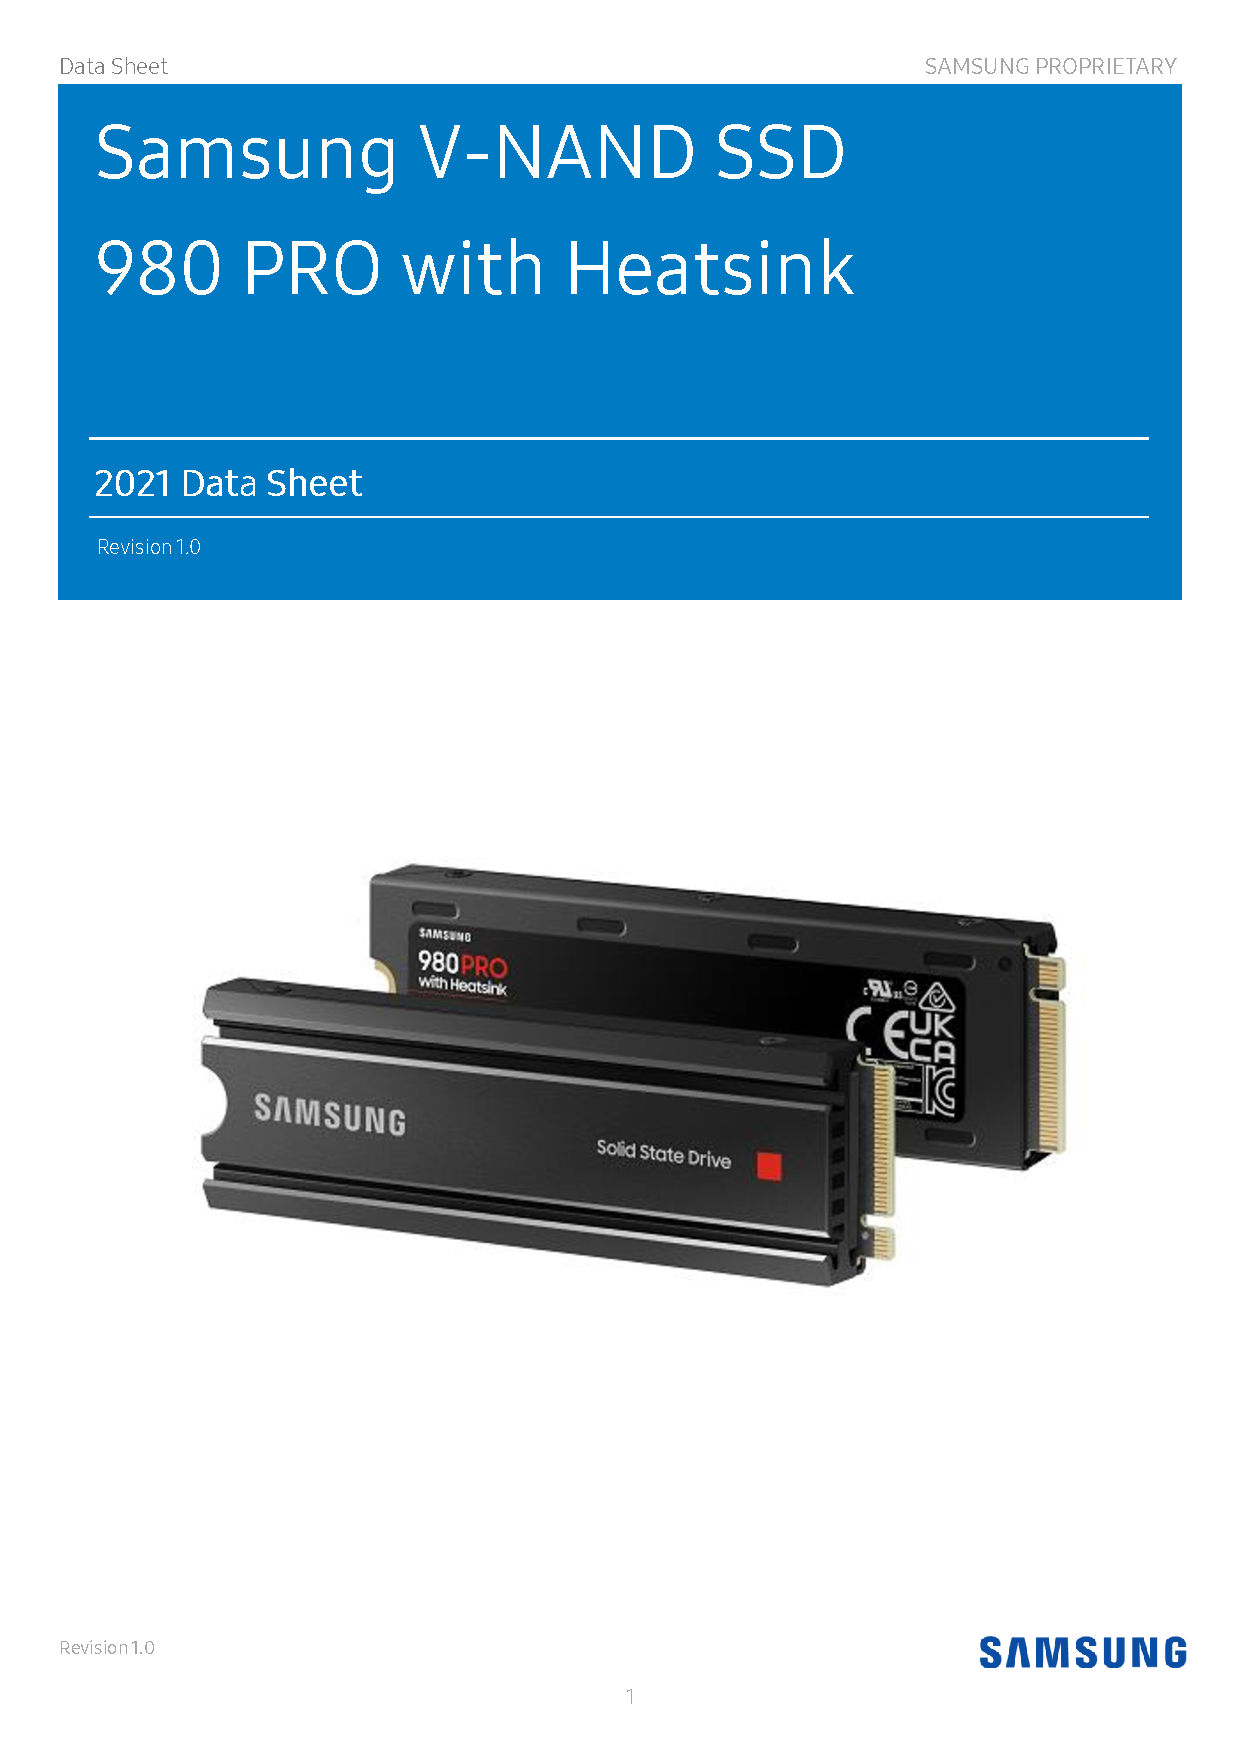
\includegraphics[trim={3cm 7cm 3cm 14cm},clip,scale=0.3,page=1]{img/Samsung_NVMe_SSD_980_PRO_with_Heatsink_Datasheet_211101.pdf} }
    \end{textblock}
    \begin{textblock}{100}(80,5)
    \uncover<4->{ \includegraphics[trim={5cm 9.6cm 1cm 3.8cm},clip,scale=0.5,page=3]{img/Samsung_NVMe_SSD_980_PRO_with_Heatsink_Datasheet_211101.pdf} }
    \end{textblock}
    \begin{textblock}{100}(68,2)
    \uncover<4->{ \textcolor{verdeuca}{\textbf{Ejemplo:}} }
    \end{textblock}
    \begin{textblock}{70}(7,12)
    \small
    \texttt{NVM} o \emph{Nonvolatile memory} son dispositivos \textbf{basados en memorias Flash} que usualmente se denominan discos de estado solido, como remplazo de los discos mecanicos.\\
    \medskip
    \uncover<2->{
    \textcolor{verdeuca}{Son mucho más rápidos, ya que no tienen tiempo de \emph{seek} ni latencia por la rotación. Adicionalmente consumen menos energía.}\\ }
    \medskip
    \uncover<3->{
    Negativamente, las celdas pueden ser escritas una \textbf{cantidad limitada de veces}, por lo que su tiempo de vida se mide en relación a la cantidad de escrituras.\\ }
    \end{textblock}
\end{frame}

\begin{frame}{Discos de estado sólido (NVM)}
    \begin{textblock}{100}(90,5) \uncover<3->{ \includegraphics[scale=0.38]{img/ssd_write-layer1.pdf} } \end{textblock}
    \begin{textblock}{100}(90,5) \uncover<4->{ \includegraphics[scale=0.38]{img/ssd_write-layer2.pdf} } \end{textblock}
    \begin{textblock}{100}(90,5) \uncover<5->{ \includegraphics[scale=0.38]{img/ssd_write-layer3.pdf} } \end{textblock}
    \begin{textblock}{100}(90,5) \uncover<6->{ \includegraphics[scale=0.38]{img/ssd_write-layer4.pdf} } \end{textblock}
    \begin{textblock}{70}(7,12)
    \small
    Las celdas de las memorias \emph{NAND} una vez escritas no pueden ser reescritas nuevamente, deben ser borradas para luego ser reescritas.\\
    \medskip
    \uncover<2->{
    \textcolor{verdeuca}{El borrado no se puede realizar sobre una celda independiente, sino se realiza por bloques de celdas.}\\ }
    \medskip
    \uncover<3->{
    \textcolor{naranjauca}{Es decir, \textbf{si queremos alterar varias celdas, debemos invalidarlas y escribir la nueva versión en otras celdas.}}\\ }
    \medskip
    \uncover<6->{
    Para mantener la relación entre las celdas físicas y lógicas, el controlador posee un \emph{flash translation layer} (FTL) que guarda esta relación.\\ }
    \medskip
    \uncover<7->{
    \textcolor{verdeuca}{La controladora además se ocupa de ejecutar un algoritmo de \emph{Garbage collection} que captura las celdas invalidas y las borra para ser reutilizadas.}\\ }
    \end{textblock}
\end{frame}

\begin{frame}{Discos de estado sólido (NVM)}
    \begin{textblock}{100}(86,10) \uncover<1->{ \includegraphics[scale=0.28]{img/gc-layer1.pdf} } \end{textblock}
    \begin{textblock}{100}(86,10) \uncover<2->{ \includegraphics[scale=0.28]{img/gc-layer2.pdf} } \end{textblock}
    \begin{textblock}{100}(86,10) \uncover<3->{ \includegraphics[scale=0.28]{img/gc-layer3.pdf} } \end{textblock}
    \begin{textblock}{100}(90,50) \uncover<4->{ \includegraphics[scale=0.45]{img/Write_Amplification_on_SSD-layer1.pdf} } \end{textblock}
    \begin{textblock}{100}(90,50) \uncover<5->{ \includegraphics[scale=0.45]{img/Write_Amplification_on_SSD-layer2.pdf} } \end{textblock}
    \begin{textblock}{100}(90,50) \uncover<6->{ \includegraphics[scale=0.45]{img/Write_Amplification_on_SSD-layer3.pdf} } \end{textblock}
    \begin{textblock}{100}(90,50) \uncover<7->{ \includegraphics[scale=0.45]{img/Write_Amplification_on_SSD-layer4.pdf} } \end{textblock}
    \begin{textblock}{100}(90,50) \uncover<8->{ \includegraphics[scale=0.45]{img/Write_Amplification_on_SSD-layer5.pdf} } \end{textblock}
    \begin{textblock}{100}(90,50) \uncover<9->{ \includegraphics[scale=0.45]{img/Write_Amplification_on_SSD-layer6.pdf} } \end{textblock}
    \begin{textblock}{70}(7,12)
    \small
    \uncover<1->{
    Los algoritmos de \emph{Garbage collection} pueden llegar a generar un efecto no deseado denominado \emph{write amplification}.\\
    \textcolor{verdeuca}{Al escribir una celda esta puede ser reescrita en otra y así sucesivamente, mientras el GC busca agrupar bloques para borrar.}\\ }
    \medskip
    \uncover<10->{
    Además puede pasar que determinados bloques sean borrados y escritos todo el tiempo, mientras otros no son modificados.\\
    \textcolor{verdeuca}{Para evitar esto se cuenta con algoritmos de \emph{Wear leveling}, que buscan distribuir el uso de los bloques en toda la memoria.}\\ }
    \medskip
    \uncover<11->{
    Adicionalmente, las memorias cuentan con un \emph{Over-provisioning}, es decir que tienen más bloques físicos que lógicos.\\
    \textcolor{verdeuca}{De esta forma pueden ayudar con espacio extra a los mecanismos mencionados.} }
    \end{textblock}
\end{frame}

\begin{frame}{Protocolos y tipos de conexión}
    \begin{textblock}{120}(35,9)
    \small
    \begin{itemize}
    \item[-]<1-> \small \textcolor{naranjauca}{Integrated Drive Electronics (IDE)}\\ \footnotesize
    Primera versión de Advanced Technology Attachment (ATA). Permitía conectar dos dispositivos como \emph{master} y \emph{slave}.
    Se implementaron diferentes estándares: EIDE (Enhanced IDE), Ultra DMA 66, Ultra DMA 100, Ultra DMA 133 desde 1986 al 2003.
    Inicialmente se integraban en placas multi-I/O, para luego terminar formando parte del \emph{motherboard}.
    \item[-]<2-> \small \textcolor{naranjauca}{Small Computer System Interface (SCSI)}\\ \footnotesize
    Es una interfaz para discos, impresoras y scaners de gran velocidad. Permite conectar diferentes buses a diferentes velocidades sobre múltiples dispositivos.
    Se utiliza principalmente en servidores y grandes sistemas. Las versiones más modernas soportan conectar y desconectar dispositivos en funcionamiento (\emph{hot plug}).
    \item[-]<3-> \small \textcolor{naranjauca}{Serial ATA (SATA)}\\ \footnotesize
    Evolución del protocolo ATA. Provee un nuevo conector físico que envia la información en serie, soportando mayor frecuencia y velocidad.
    Además fue diseñado para \emph{hot plug} a diferencia de IDE.
    \item[-]<4-> \small \textcolor{naranjauca}{NVM Express o Non-Volatile Memory Express (NVMe)}\\ \footnotesize
    Es un protocolo de comunicación especialmente diseñado para trabajar con memorias flash usando interfaces PCIe.
    Tiene en cuenta la ventaja de la operación en paralelo de los dispositivos de estado solido.
    \end{itemize}
    \end{textblock}
    \begin{textblock}{120}(5,10)
    \uncover<1->{ 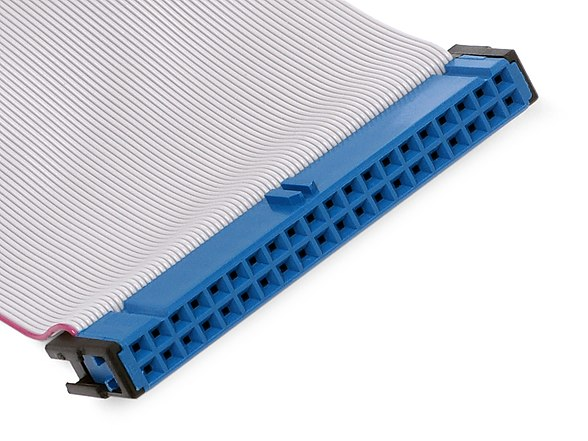
\includegraphics[width=3cm]{img/IDE.jpg} } \\
    \uncover<2->{ 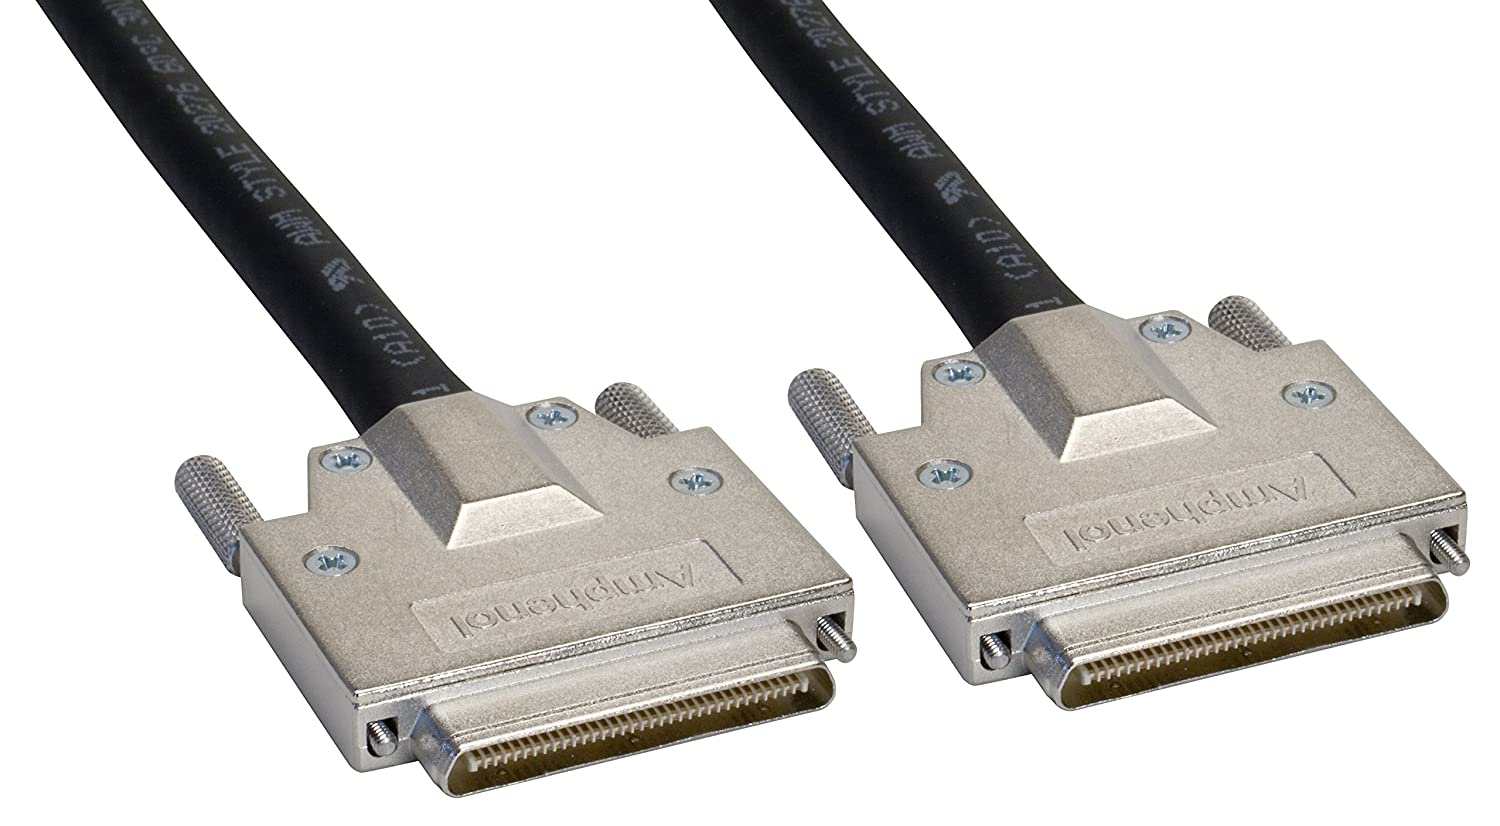
\includegraphics[width=3cm]{img/SCSI.jpg} } \\
    \uncover<3->{ 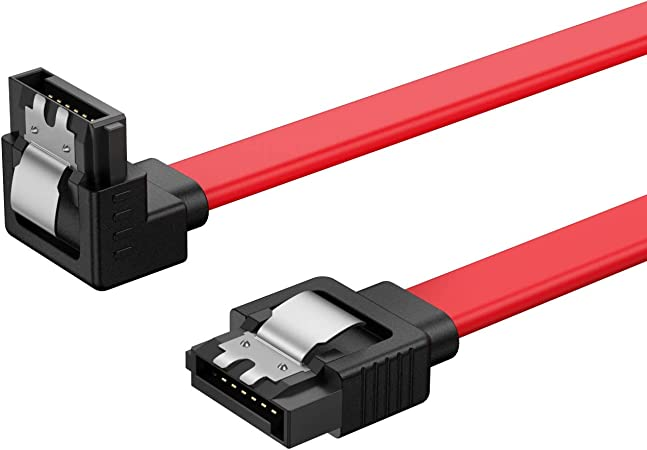
\includegraphics[width=3cm]{img/SATA.jpg} } \\
    \uncover<4->{ 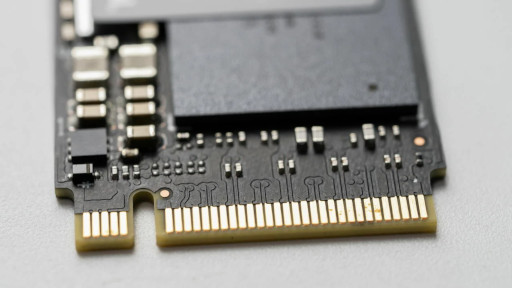
\includegraphics[width=3cm]{img/NVMe.jpg} }
    \end{textblock}
\end{frame}

% Cloud Storage Basics
% Caesar Wu, Rajkumar Buyya, in Cloud Data Centers and Cost Modeling, 2015
% 12.4.2.1 IDE/ATA/parallel ATA or PATA
%     TA Version	Standard	Year	Speed	Key Features
% IDE	ATA-1	1986		Pre-standard
% ATA	1994		PIO (programmed IO) modes 0–2 multiword Direct Memory Access (DMA) 0
% EIDE (Enhanced IDE)	ATA-2	1996	16 MB/s	PIO mode 3–4 multiword DMA mode 1–2, Logical Block Address (LBA)
% ATA-3	1997	16 MB/s	Self-Monitoring Analysis and Reporting Technology (SMART)
% ATA/ATAPI-4	1998	33 MB/s	Ultra DMA modes 0–2, Cyclic Redundancy Code (CRC) queuing, 8-wire
% Ultra DMA 66	ATA/ATAPI-5	2000	66 MB/s	Ultra DMA mode 3–4
% Ultra DMA 100	ATA/ATAPI-6	2002	100 MB/s	Ultra DMA mode 5, 48-bit LBA
% Ultra DMA 133	ATA/ATAPI-7	2003	133 MB/s	Ultra DMA mode 6

\begin{frame}{Almacenamiento Masivo}
   \begin{textblock}{100}(30,7)
    \uncover<1->{ 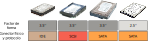
\includegraphics[scale=0.65]{img/tecnologiaHDD.pdf} }
    \end{textblock}
    \begin{textblock}{100}(20,37)
    \uncover<1->{ 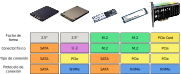
\includegraphics[scale=0.65]{img/tecnologiaSSD.pdf} }
    \end{textblock}
\end{frame}

\begin{frame}{Formateo de bajo nivel}
    Inicialmente los discos no tienen ningún formato específico.\\
    Ni siquiera cuentan con la construcción lógica de un sector.\\
    \bigskip
    Parar esto se realiza el \textbf{formateo de bajo nivel}.\\
    \medskip
    \begin{center}
    \begin{tabular}{|c|c|c|}
    \hline
    Encabezado & \ \ \ \ \ \ \ \ \ \ \ \ \ \ ... Datos ... \ \ \ \ \ \ \ \ \ \ \ \ \ \ & Código de correción de errores\\
    \hline
    \end{tabular}
    \end{center}
    \pause
    \bigskip
    \textcolor{verdeuca}{
    Consiste en construir una estructura con información del sector y disco, datos e información para la correción de errores.\\
    Esta última, permite no solo detectar, sino arreglar errores que puedan tener los datos.}\\
    \medskip
    El tamaño de los datos para un sector puede ser de entre 512 bytes a 4KB.\\
\end{frame}

\begin{frame}{Particiones en un disco}
    Los discos suelen ser particionados tanto para ordenar la información, como por razones funcionales.
    \textbf{Cada partición puede contener un determinado sistema de archivos.}\\
    \bigskip
    \textcolor{gray}{Algunas aplicaciones especiales como los motores de bases de datos o el espacio de intercambio (\emph{swap}) no necesitan un formato especial.}\\
    \bigskip
    \pause
    \textcolor{naranjauca}{\textbf{Particiones}}\\
    Las particiones que se utilizarán para sistemas de archivos, se formatean escribiendo conjuntos de sectores de \emph{metadata} que permite determinar donde se guarda cada archivo.\\
    \bigskip
    \pause
    \textcolor{naranjauca}{\textbf{Sector de arranque}} o \textcolor{naranjauca}{MBR (\textit{Master-boot Record})}\\
    Es un sector distingido del disco que almacena datos sobre la tabla de particionado y rutinas de código básicas que sirven como el primer paso en la carga del sistema operativo.
    % Editor de particiones
    % FIGURA boot-loader del MBR
\end{frame}

\begin{frame}{RAID (Arreglo Redundante de Discos Económicos)}
    El termino \textbf{RAID} fue acuñado en 1988 en el paper ``\emph{A Case for Redundant Arrays of Inexpensive Disks (RAID)}'' para luego hacer referencia a ``\emph{redundant array of independent disks}''.\\
    La idea es utilizar un \textcolor{verdeuca}{\textbf{conjunto de discos}} físicos para construir un único volumen lógico, configurando además un determinado \textcolor{verdeuca}{\textbf{grado de replicación}} de los datos.\\
    \bigskip
    \pause
    Existen distintos niveles de RAID que dependen de como los datos son almacenados y replicados en los discos.\\
    \bigskip
    El soporte para RAID puede ser tanto por \textcolor{verdeuca}{\textbf{hardware}}, mediante placas especiales que controlan el acceso a los discos y su replicación, como por \textcolor{verdeuca}{\textbf{software}}, delegando toda la tarea de administración al sistema operativo.\\
    \bigskip
    \pause
    \textcolor{verdeuca}{El objetivo de un RAID es tener mayor espacio de almacenamiento que en discos individuales, mejor rendimiento balanceando la carga y mejor el soporte ante fallas.}
\end{frame}

\begin{frame}{RAID (Arreglo Redundante de Discos Económicos)}
    \begin{center}
    \begin{tabular}{lccc}
            & \textbf{Mínimo de discos} & \textbf{Protección de datos} & \textbf{Capacidad utilizada} \\ \hline
    \uncover<1->{ \textcolor{naranjauca}{\textbf{RAID 0}} (striping)      & 2 & Sin protección    & 100\% \\ }
    \uncover<2->{ \textcolor{naranjauca}{\textbf{RAID 1}} (espejado)      & 2 & Error en un disco & 50\% \\ }
    \uncover<3->{ \textcolor{naranjauca}{\textbf{RAID 5}} (paridad)       & 3 & Error en un disco & 66\% a 90\% \\ }
    \uncover<4->{ \textcolor{naranjauca}{\textbf{RAID 6}} (doble paridad) & 3 & Error en dos discos & 50\% a 80\% \\ }
    \uncover<5->{ \textcolor{naranjauca}{\textbf{RAID 10}} (striping espejado) & 4 & Error en un disco & 50\% \\ } 
    \end{tabular}
    \vspace{-0.5cm}
    \end{center}
    \begin{center}
    \uncover<1->{ \includegraphics[scale=1.2]{img/raid-layer1.pdf} } \hspace{-3cm} 
    \uncover<2->{ \includegraphics[scale=1.2]{img/raid-layer2.pdf} } \hspace{-3cm}  
    \uncover<3->{ \includegraphics[scale=1.2]{img/raid-layer3.pdf} } \\ \vspace{0.2cm}
    \uncover<4->{ \includegraphics[scale=1.2]{img/raid-layer4.pdf} } \hspace{1cm} 
    \uncover<5->{ \includegraphics[scale=1.2]{img/raid-layer5.pdf} }
    \end{center}
\end{frame}

\begin{frame}[fragile]
    \frametitle{Bibliografía}
    \begin{itemize}
        \setlength\itemsep{0.5cm}
        \item[-] \small Silberschatz, ``Fundamentos de Sistemas Operativos'', 7ma Edición, 2006.\\
        \begin{itemize}
            \item \textbf{Capítulo 12 - Estructura de almacenamiento masivo}, páginas 407-410 y 412-423
        \end{itemize}
        \item[-] \small Silberschatz, ``Operating System Concepts'', 10th Edition, 2018.\\
        \begin{itemize}
            \item \textbf{Chapter 11 - Mass-Storage Structure}, páginas 452-454 y 461-462
        \end{itemize}
    \end{itemize}
\end{frame}

\begin{frame}[plain]
    \begin{center}
    \vspace{2cm}
    \huge ¡Gracias!\\
    \vspace{2cm}
%     \normalsize Recuerden leer los comentarios adjuntos\\ en cada clase por aclaraciones.
    \end{center}
\end{frame}

\end{document}
